\documentclass[sigplan,10pt,review,anonymous]{acmart}\settopmatter{printfolios=true,printccs=false,printacmref=false}
  \usepackage{graphicx}
  \usepackage{listings}
    %% For double-blind review submission, w/ CCS and ACM Reference
    %\documentclass[sigplan,10pt,review,anonymous]{acmart}\settopmatter{printfolios=true}
    %% For single-blind review submission, w/o CCS and ACM Reference (max submission space)
    %\documentclass[sigplan,10pt,review]{acmart}\settopmatter{printfolios=true,printccs=false,printacmref=false}
    %% For single-blind review submission, w/ CCS and ACM Reference
    %\documentclass[sigplan,10pt,review]{acmart}\settopmatter{printfolios=true}
    %% For final camera-ready submission, w/ required CCS and ACM Reference
    %\documentclass[sigplan,10pt]{acmart}\settopmatter{}
    
    
    %% Conference information
    %% Supplied to authors by publisher for camera-ready submission;
    %% use defaults for review submission.
    \acmConference[PL'17]{ACM SIGPLAN Conference on Programming Languages}{January 01--03, 2017}{New York, NY, USA}
    \acmYear{2017}
    \acmISBN{} % \acmISBN{978-x-xxxx-xxxx-x/YY/MM}
    \acmDOI{} % \acmDOI{10.1145/nnnnnnn.nnnnnnn}
    \startPage{1}
    
    %% Copyright information
    %% Supplied to authors (based on authors' rights management selection;
    %% see authors.acm.org) by publisher for camera-ready submission;
    %% use 'none' for review submission.
    \setcopyright{none}
    %\setcopyright{acmcopyright}
    %\setcopyright{acmlicensed}
    %\setcopyright{rightsretained}
    %\copyrightyear{2017}           %% If different from \acmYear
    
    %% Bibliography style
    \bibliographystyle{ACM-Reference-Format}
    %% Citation style
    %\citestyle{acmauthoryear}  %% For author/year citations
    %\citestyle{acmnumeric}     %% For numeric citations
    %\setcitestyle{nosort}      %% With 'acmnumeric', to disable automatic
                                %% sorting of references within a single citation;
                                %% e.g., \cite{Smith99,Carpenter05,Baker12}
                                %% rendered as [14,5,2] rather than [2,5,14].
    %\setcitesyle{nocompress}   %% With 'acmnumeric', to disable automatic
                                %% compression of sequential references within a
                                %% single citation;
                                %% e.g., \cite{Baker12,Baker14,Baker16}
                                %% rendered as [2,3,4] rather than [2-4].
    
    
    %%%%%%%%%%%%%%%%%%%%%%%%%%%%%%%%%%%%%%%%%%%%%%%%%%%%%%%%%%%%%%%%%%%%%%
    %% Note: Authors migrating a paper from traditional SIGPLAN
    %% proceedings format to PACMPL format must update the
    %% '\documentclass' and topmatter commands above; see
    %% 'acmart-pacmpl-template.tex'.
    %%%%%%%%%%%%%%%%%%%%%%%%%%%%%%%%%%%%%%%%%%%%%%%%%%%%%%%%%%%%%%%%%%%%%%
    
    
    %% Some recommended packages.
    \usepackage{booktabs}   %% For formal tables:
                            %% http://ctan.org/pkg/booktabs
    \usepackage{subcaption} %% For complex figures with subfigures/subcaptions
                            %% http://ctan.org/pkg/subcaption
    
    
    \begin{document}
    
    %% Title information
    \title{Simplifying the Programming of Microcontroller-based Devices}         %% [Short Title] is optional;
                                            %% when present, will be used in
                                            %% header instead of Full Title.
    \subtitle{Microsoft MakeCode and Lancester University Teams}                     %% \subtitle is optional

    
    %% Author information
    %% Contents and number of authors suppressed with 'anonymous'.
    %% Each author should be introduced by \author, followed by
    %% \authornote (optional), \orcid (optional), \affiliation, and
    %% \email.
    %% An author may have multiple affiliations and/or emails; repeat the
    %% appropriate command.
    %% Many elements are not rendered, but should be provided for metadata
    %% extraction tools.
    
    %% Author with single affiliation.
    \author{First1 Last1}
    \authornote{with author1 note}          %% \authornote is optional;
                                            %% can be repeated if necessary
    \orcid{nnnn-nnnn-nnnn-nnnn}             %% \orcid is optional
    \affiliation{
      \position{Position1}
      \department{Department1}              %% \department is recommended
      \institution{Institution1}            %% \institution is required
      \streetaddress{Street1 Address1}
      \city{City1}
      \state{State1}
      \postcode{Post-Code1}
      \country{Country1}                    %% \country is recommended
    }
    \email{first1.last1@inst1.edu}          %% \email is recommended
    
    %% Author with two affiliations and emails.
    \author{First2 Last2}
    \authornote{with author2 note}          %% \authornote is optional;
                                            %% can be repeated if necessary
    \orcid{nnnn-nnnn-nnnn-nnnn}             %% \orcid is optional
    \affiliation{
      \position{Position2a}
      \department{Department2a}             %% \department is recommended
      \institution{Institution2a}           %% \institution is required
      \streetaddress{Street2a Address2a}
      \city{City2a}
      \state{State2a}
      \postcode{Post-Code2a}
      \country{Country2a}                   %% \country is recommended
    }
    \email{first2.last2@inst2a.com}         %% \email is recommended
    \affiliation{
      \position{Position2b}
      \department{Department2b}             %% \department is recommended
      \institution{Institution2b}           %% \institution is required
      \streetaddress{Street3b Address2b}
      \city{City2b}
      \state{State2b}
      \postcode{Post-Code2b}
      \country{Country2b}                   %% \country is recommended
    }
    \email{first2.last2@inst2b.org}         %% \email is recommended
    
    
    %% Abstract
    %% Note: \begin{abstract}...\end{abstract} environment must come
    %% before \maketitle command
    \begin{abstract}
    Text of abstract \ldots.
    \end{abstract}
    
    %% Keywords
    %% comma separated list
    \keywords{keyword1, keyword2, keyword3}  %% \keywords are mandatory in final camera-ready submission
    
    
    %% \maketitle
    %% Note: \maketitle command must come after title commands, author
    %% commands, abstract environment, Computing Classification System
    %% environment and commands, and keywords command.
    \maketitle
    
    Microcontrollers, traditionally the workhorses of embedded systems, have become 
central to efforts in making and education. For example, the Arduino project, 
started in 2003, created a printed circuit board (the Uno) based on the 8-bit Atmel 
AVR microcontroller unit that makes most of the its I/O pins available via headers on 
the board.  Hardware modules (shields) may be connected to the main board to extend its capability. 
The Arduino ecosystem, based on an open hardware design, has grown tremendously in the past 15 years, 
with the support of companies such as Adafruit Industries and Sparkfun Electronics, to name a few.

What has not changed much in this time is the way these boards are programmed.  
The C and C++ programming languages are the primary way to program microcontrollers. 
This is not a huge surprise, given the low-level nature of microcontroller programming, 
where direct access to the hardware is the order of the day. There generally is no operating 
system running on such boards, as they have very little RAM (2K for the Uno, for example) and 
lack memory protection hardware.  What is more surprising about the Arduino platform is that:
\begin{itemize}
\item it encourages the use of polling by the end-user as the primary way to interact with sensors, 
which leads to monolithic sequential programs;
\item its IDE lacks any code “intellisense” or common interactive features of modern IDEs;
\item it loads code onto the microcontroller using 1980s era bootloader technology.
\end{itemize}
As a result, it is not simple to get started with systems based on Arduino, of which there are many. 
On the other hand, on the web we find many excellent environments for introducing programming to beginners. 
Visual block-based editors such as Scratch and Blockly allow the creation of programs without the possibility 
of syntax errors. HTML and JavaScript allow a complete programming experience to be delivered as an interactive 
web application, including editing with intellisense, code execution and debugging. (While the Arduino IDE recently 
has been ported to the web, it lacks many of the above features and requires a web connection to a server which runs 
a C/C++ compile tool chain to compile user code.) The programming models associated with these environments are 
generally event-based, freeing the user from the tyranny of polling.

We present a new programming platform that bridges the gap between the worlds of the microcontroller and the web app. 
The goals of the platform are three-fold:
\begin{itemize}
\item[1.] make it simple to program microcontrollers using an interactive web app that works when offline;
\item[2.] allow a user’s compiled program to be easily installed on a microcontroller;
\item[3.] support the addition of new of software/hardware components to a microcontroller.
\end{itemize}
The platform, MCCU, consists of three major components (MakeCode, CODAL and UF2), which we now describe. 
The MakeCode web app (see www.makecode.com) supports both visual block-based programming and text-based programming 
using TypeScript, a gradually-typed superset of JavaScript, with the ability to convert between the two representations. 
The web app supports in-browser execution, via a device simulator, and compilation to machine code, linking against the 
pre-compiled CODAL C++ runtime to produce a binary for execution on an microcontroller (either 8-bit AVR and 16-bit ARM 
Thumb instruction set). No C/C++ compiler is invoked for a compilation of user code. The result of compilation is a 
binary file that is “downloaded” from the web app to the user’s computer. The USB flashing format (UF2) makes copying 
of the binary file to the device, mounted as removable flash drive, fast and reliable, across all major operating systems. 
Once the web app has been loaded, all the above functionality works offline (i.e., if the host machine loses its connection 
to the internet).

The main innovations of MCCU are:
\begin{itemize}
\item The design and implementation of MakeCode, which bridges the worlds of JavaScript and C++, 
      enabling beginners to get started programming microcontrollers from any modern web browser and enabling 
      hardware vendors to innovate and safely add new components to the mix. 
\item Static TypeScript, a statically-typed subset of TypeScript for fast execution on low-memory devices and a simple model for linking against pre-compiled C++; Static TypeScript also can be used to write safe and performant device driver code.
\item CODAL, the Component-oriented Device Abstraction Layer, maps each hardware component to one or more software components that communicate over a message bus and schedule event handlers to run non-preemptively on fibers. 
\item The USB Flashing Format (UF2), a file format designed for flashing microcontrollers over the Mass Storage Class (removable USB pen drive) protocol.  This new file format greatly speeds the installation of user programs and is robust to difference in operating systems.
\end{itemize}


MCCU combines these innovations in programming languages, language runtime, and code loading to make a simple 
programming experience for the end user.  Through its support for Static TypeScript and a foreign function 
interface to C++, MCCU makes it easy for hardware manufacturers to share their C++ components with a wider audience.  
All of MCCU’s components are open source under the MIT license, as detailed below. 

MCCU targets can be seen at www.makecode.com, where the MakeCode web app for a variety of boards is available, 
including the micro:bit (a Nordic nRF51822 microcontroller with Cortex-M0 processor, 16K RAM), Adafruit’s Circuit 
Playground Express (CPX: an Atmel SAMD21 microcontroller with Cortex-M0 processor, 16K RAM), and the Arduino Uno 
(Uno: an Atmel ATmega328 microcontroller with AVR processor, 2K RAM). 

We encourage the reader to choose a board and experiment with programming it, using the simulator to explore many of each board’s features, 
to appreciate the qualitative aspects of MCCU: its simplicity and ease of use.  In this paper, we will evaluate quantitative aspects of MCCU: 
compilation speed, code size, and runtime performance.  We evaluate:
\begin{itemize}
\item the compile time of Static TypeScript compile/link of user code (to machine code) with respect to the GCC-based C/C++ toolchain, as well as the size of the resulting executable;
\item the time to load code onto a microcontroller using UF2, compared to standard bootloaders; 
\item The performance of a set of small benchmarks, written in both Static TypeScript and C++, compiled with the MakeCode and GCC-based toolchains, as well as the performance of device drivers written in Static TypeScript compared to their C++ counterparts.
\end{itemize}
[evaluate with respect to the popular Arduino toolset, for boards with 8-bit (AVR) and 32-bit (Cortex-M0) microcontrollers. 
Summary of evaluation]

MCCU is open source on www.github.com. The MakeCode framework is at microsoft/pxt (PXT is previous codename of MakeCode). 
MakeCode targets for the three previously mentioned boards are at microsoft/pxt-microbit, microsoft/pxt-adafruit and 
microsoft/pxt-arduino-uno. The latter two targets make use of a common set of MakeCode libraries (packages) at 
microsoft/pxt-common-packages. [pxt-monaco, pxt-blockly].   Many other MakeCode packages, developed by Microsoft and 
hardware partners [details later]. A few examples: XYZ.  

%Lancaster University githubs:
%•	https://github.com/lancaster-university/codal-core
%•	https://github.com/lancaster-university/codal 
%•	micro:bit DAL: https://github.com/lancaster-university/microbit-dal, predecessor of CODAL 
%UF2 githubs
%•	Specification: https://github.com/microsoft/uf2 
%•	SAMD21: https://github.com/microsoft/uf2-samd21
%•	Atmega32UP???

The rest of this paper is organized as follows. Section 2 presents the design and implementation of the MakeCode framework. Section 3 describes Static TypeScript Overview of the paper: MakeCode, Static TypeScript, CODAL, UF2, Evaluation, Related Work, Conclusion and Future Directions. 

    \section{MakeCode: Design and Implementation}
\label{sec:makecode}

\begin{figure}[t]
    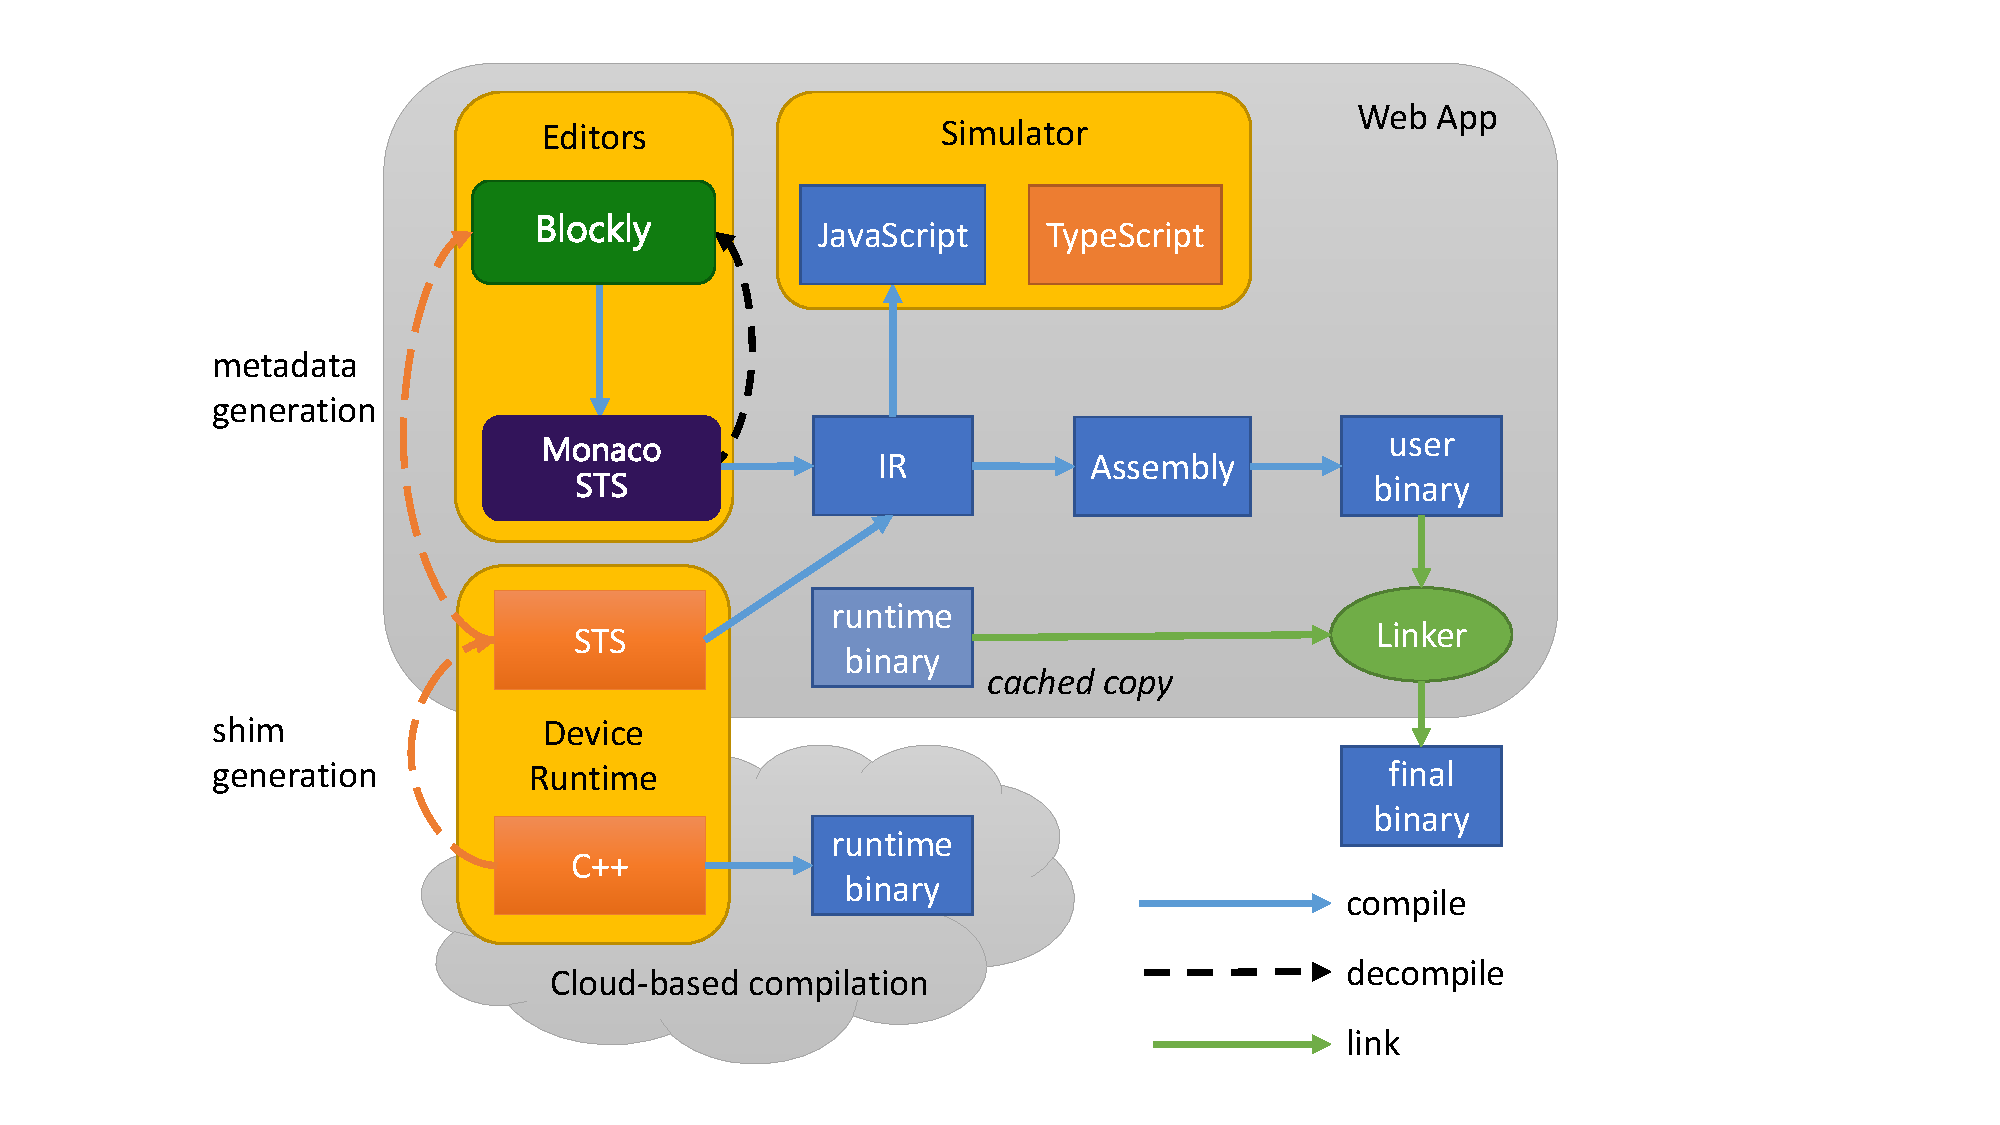
\includegraphics[width=4.5in]{diagrams.pdf}
\caption{\label{fig:makecode}MakeCode Architecture}
\end{figure}

The MakeCode web app encapsulates all the components needed to deliver a programming experience 
for microcontroller-based devices, free of the need for a C++ compiler for the compilation of user 
code, as shown in Figure~\ref{fig:makecode}. 
The web app is written in TypeScript. The web app also incorporates the TypeScript compiler and 
language service (www.typescriptlang.org) which are used in several ways, as detailed below. 
The remaining subsections describe the parts of Figure~\ref{fig:makecode}.

\subsection{Device Runtime and Shim Generation}

A MakeCode target is defined, in part, by its device runtime, which can be a combination of C++ 
and Static TypeScript (STS) code. The C++ runtime for the target microcontroller is precompiled 
and stored in the cloud. The C++ runtime binary is cached in the HTML5 application cache (with 
other assets) so that the web app can function when the browser is offline. Additional runtime
components may be authored in STS, which allows the device runtime to be updated without the need
for any C++ programming, and permits components of the device runtime to be shared by both the device
and simulator runtimes.  We will describe later how elements of the C++ runtime are exposed to STS
(via automated shim generation). The ability to author the device runtime in both STS and C++ is
a unique aspect of MakeCode's design.

Whether runtime components are authored in C++ or STS, all runtime APIs are exposed as fully-typed
TypeScript definitions (for runtime components written in TypeScript) or declarations (for runtime
components written in C++). A full-typed runtime improves the end-user experience by making it easier
to discover APIs; it also enables the type inference provided by the TypeScript compiler to infer types
for (unannotated) user code.

MakeCode supports a simple foreign function interface from TypeScript to C++ based on namespaces,
enumerations, functions, and basic type mappings. MakeCode uses top-level namespaces (in both C++ and
TypeScript) to organize sets of related functions.  Preceding a C++ namespace, enumeration, or function
with \emph{//\%} indicates that MakeCode should map the C++ construct to TypeScript.
Within the \emph{//\%} comment, attributes are used to define the visual appearance for that
language construct, such as for the led namespace in the micro:bit target:

\begin{lstlisting}
//% color=#5C2D91 weight=97 icon="\uf205"
namespace led { 
...
\end{lstlisting}

Here is the C++ file defining the micro:bit's led namespace and its functions:
\begin{center}
\url{https://github.com/Microsoft/pxt-microbit/blob/master/libs/core/led.cpp}
\end{center}

Mapping of functions and enumerations between C++ and TypeScript is straightforward. 
Here's an example of the C++ function plot in the led namespace that wraps a more
complex function call of the underlying device runtime to set/plot an LED in the micro:bit display:

\begin{lstlisting}
//% blockId=device_plot block="plot|x %x|y %y"
//% x.min=0 x.max=4 y.min=0 y.max=4
void plot(int x, int y) {
    uBit.display.image.setPixelValue(x, y, 1);
}
\end{lstlisting}

We'll describe the attribute definitions in the \emph{//\%} comment in the next section. 
MakeCode uses a  TypeScript declaration file to describe the TypeScript elements corresponding
to C++ namespaces, enumerations and functions.  We call such files shim files.
Since the C++ plot function is preceded by a \emph{//\%} comment, 
MakeCode adds the following TypeScript declaration to the shim file (shims.d.ts) and copies
over the attribute definitions in the comment. MakeCode also adds an attribute definition mapping
the TypeScript shim to its C++ function (shim=led::plot):

\begin{lstlisting}
//% blockId=device_plot block="plot|x %x|y %y
//% x.min=0 x.max=4 y.min=0 y.max=4 shim=led::plot
function plot(x: number, y: number): void;
\end{lstlisting}

Here is the shim file generated from the annotated C++ sources for the micro:bit device runtime: 
\begin{center}
\url{https://github.com/Microsoft/pxt-microbit/blob/master/libs/core/shims.d.ts}
\end{center}

To support the foreign function interface, MakeCode defines a mapping between C++ and TypeScript types.
Boolean and void have straightforward mappings from C++ to TypeScript (bool → boolean, void → void). 
As JavaScript only supports number, which is a C++ float/double, MakeCode uses TypeScript's support
for type aliases to name the various C++ integer types commonly used for microcontroller programming
(int $\rightarrow$ int32, unsigned $\rightarrow$  uint32, short $\rightarrow$ int16, 
byte $\rightarrow$ uint8, sbyte $\rightarrow$ int8).  This is particularly
useful for saving space on 8-bit architectures such as the AVR. 

MakeCode supports both untagged and tagged integers (described more later).  Under the untagged strategy,
a JavaScript number is interpreted as a C++ int by default, while the tagged strategy allows both
interpretation as integer and double (with an optimization to convert from integer to double, as required).  
MakeCode includes reference counted C++ types for strings (StringData*) and parameterless lambdas (Action).

These C++ types are mapped to the TypeScript types string and ()=>void, respectively.
MakeCode allows a set of C++ functions with the same first parameter (of type Foo) to be
exposed as a TypeScript interface Foo as follows: this set of C++ functions must be grouped
inside a namespace of the name FooMethods.  See, for example, how a C++ buffer abstraction is exposed:

\begin{center}
\url{https://github.com/Microsoft/pxt-microbit/blob/master/libs/core/buffer.cpp}
\end{center}

You can find the resulting TypeScript Buffer interface in the shim file for the micro:bit
(already referenced above). 

\subsection{Block Metadata Generation}

Both C++ and TypeScript APIs can be specially annotated (minimally via 
\emph{//\% block}) so that the MakeCode compiler generates the needed
Blockly metadata to expose an API as a visual block. So, to expose the previously
encountered plot function as a visual block (as well as a TypeScript function), one simply needs:
\begin{lstlisting}
//% block
void plot(int x, int y) { . . . }
\end{lstlisting}

Additional attribute definitions can provide text descriptions for the block, project function
parameters (thus simplifying the API available via Blockly), and describe other visual/functional
characteristics of the block.  MakeCode uses the types of function parameters to select appropriate
Blockly widgets.  For example, an enumeration is represented by a dropdown menu in blocks.
For more information on the block-specific annotations, see 
\url{https://makecode.com/defining-blocks}. 
MakeCode's support for Blockly means that for the common case, the target developer doesn't need
to know anything about the Blockly framework.  For more sophisticated needs, one can directly access
the Blockly framework. 

\subsection{Editors and Code Conversion}

MakeCode uses the Blockly (\url{https://github.com/google/blockly}) and Monaco 
(\url{https://github.com/Microsoft/monaco-editor}) editors to allow the user to code with
visual blocks or TypeScript. The editing experience is parameterized by the full-typed device
runtime, which provides a set of categorized APIs to the end-user, based on namespaces, as
previously described. These APIs are visible in both editors via a toolbox to the immediate
left of the programming area. The Blockly and Monaco toolboxes show the same set of APIs, to
help in transition from coding with blocks to coding with JavaScript. More advanced TypeScript
APIs can be discovered in Monaco via code intellisense.

The Blockly program representation is compiled to Static TypeScript in a syntax-directed manner
(see \url{https://github.com/Microsoft/pxt/tree/master/pxtblocks}). A key issue is the need for
type inference on the Blockly representation, as variables generally are defined and used without
being declared in Blockly. MakeCode uses a simple unification-based type inference to assign a
unique type to each variable.  In the future, we expect to use TypeScript's type inference instead
and eliminate the need for separate type inference over the Blockly representation. 
TypeScript supports programming constructs that are not available in Blockly, such as classes.
Such constructs are converted into grey uneditable blocks in Blockly, with the construct's program
text intact. This means MakeCode always can decompile a TypeScript program to Blockly and then recover
the program text of the grey blocks when converting from Blockly back to TypeScript
 (see \url{https://github.com/Microsoft/pxt/blob/master/pxtcompiler/emitter/decompiler.ts}). 

\subsection{Compilation Pipeline}

MakeCode first invokes the TypeScript language service to perform type inference and type checking on the 
user's program, using the TypeScript declaration files for the device runtime.   It then checks that the
user's program is within the STS subset through additional syntactic and type checks over the adorned
abstract syntax tree (AST) produced by the language service (detailed in Section XYZ).  Assuming all the
above checks pass, MakeCode then performs tree shaking and compilation of the AST of the user code and
device runtime to an intermediate representation (IR) that makes explicit: labelled control flow among a
sequence of instructions with conditional and unconditional jumps; heap cells; field accesses; store operations,
and reference counting.

There are two backends for code generation from the IR. The first backend simply generates JavaScript,
for execution against the simulator runtime.  The other backend generates assembler, parameterized by a
processor description.  Currently supported processors include ARM's Cortex class (Thumb instructions)
and Atmel's Atmega class (AVR instructions). A separate assembler, also parameterized by an instruction
encoder/decoder, generates machine code. Finally, a linker completes the compile chain by resolving
references to the driver runtime in the user's program, producing a binary executable. The compiler chain
can be found at \url{https://github.com/Microsoft/pxt/tree/master/pxtcompiler/emitter} and 
\url{https://github.com/Microsoft/pxt/tree/master/pxtlib/emitter}.

\subsubsection{Asynchronous Functions}

A key part of the compilation process is to allow users to call async functions (identified through
the \emph{//\% async} annotation) as if they were regular (blocking) functions.  This is done by
compiling each function so that it can be suspended (at the return of a call) and later resumed (at the same point). 
The default behavior at a suspension point is to immediately resume execution.  If a call is to an async function then
the default behavior is overridden by the compiler, which suspends execution of the current function. Upon completion
of the async function call, the current function then is resumed.    This feature greatly simplifies the JavaScript-based
programming model which relies on promises to achieve asynchronous execution, breaking up sequential (blocking) code into
a series of event handlers.  The JavaScript-based simulator runtime uses promises to achieve asynchronous execution in a
single-threaded context, but these promises are hidden from the end user.    The CODAL C++ device runtime supports fibers
with the ability to pause, so for compilation to a device, the compiler simply emits a call to pause at a suspension point. 

\subsubsection{Untagged and Tagged Strategies}

The MakeCode compiler supports the Static TypeScript language subset described in Section X, with two compilation
strategies: untagged and tagged. 
\emph{TODO}
Untagged compilation strategy
No support for doubles. 32-bit integers (signed only). Use static type system to distinguish between integers and references.
No runtime support.  Not fully compatible with JavaScript semantics. Null = Undefined = 0 = default integer value.  Support for
different integer sizes using type aliases (this is used for AVR). 
Tagged compilation strategy
In the tagged strategy, numbers are either tagged 31-bit signed integers, or if they do not fit, boxed doubles. Code generation
to check tag bit. Special constants like false, null and undefined are given special values and can be distinguished. Fully
compatible with JavaScript semantics (number, null, undefined).   Can accommodate a richer type system. 

\subsection{Simulator}

A MakeCode target can provide an alternate TypeScript implementation for each API in the device runtime, for use in the device
simulator. As this code runs in the web browser (not on the actual device) and manipulates the DOM, the developer is free to
use all of TypeScript/JavaScript's features. (As an aside, MakeCode also support ``simulator-only'' targets that have no 
associated device; in these cases, the ``device runtime'' is defined solely by the simulator APIs.) 
The simulator allows the user to experience the basic functions of the device in the browser and to test their code
before deploying it to the actual device. The simulator has proxy widgets for sensors such as accelerometer (mouse motion),
temperature and light, allowing the user to control the sensor's value.  The simulator only provides basic functionality
and is far from a complete device emulation.   For example, it is not possible for the user to simultaneously modify two
inputs to the simulated device, while it is possible with the actual device (i.e., shaking it to change the accelerometer
reading while pushing one of the device's buttons).

MakeCode provides various components to make device-based simulators easier to build: board, parts, wiring, etc.

\subsection{Packages and Custom Editors}

Packages are MakeCode's dynamic/static library mechanism for extending a target (by adding new code/data to the device
and simulator runtimes, as well as accompanying documentation). The following package extends the micro:bit target so
that the micro:bit can drive a NeoPixel strip of RGB LEDs: \url{https://github.com/Microsoft/pxt-neopixel}. To see how this
package is surfaced to the end-user, visit \url{http://makecode.microbit.org/} and select the ``Add Package'' option from the
gear menu; you will see the package ``neopixel'' listed in the available options. If you click on it, a new block category
named ``Neopixel'' will be added to the editor. In this scenario, PXT dynamically loads the (white listed) neopixel 
package directly from GitHub, compiles it and incorporates it into the web app. Packages also can be bundled with a web
app (the analog of static linking).  

Hardware partners already have started to create MakeCode packages for the micro:bit.
Seeed Studio (\url{https://www.seeedstudio.com/}) has created packages to add its Grove components to a micro:bit.
Grove components are accessed via the I2C serial protocol, supported by the micro:bit device runtime.
All micro:bit packages for the Grove components are authored in Static TypeScript (gesture, ultrasonic-ranger,
4-digital-display, two-led-matrix). These packages can be found under GitHub user ``Tinkertanker'', prefixed with
``pxt-''. Sparkfun has created MakeCode packages for its micro:bit shields (GitHub user ``sparkfun'').

% https://github.com/Tinkertanker/pxt-ssd1306-microbit
% https://github.com/Tinkertanker/pxt-ir-microbit 
% https://github.com/Tinkertanker/pxt-ky040-microbit
% https://github.com/Tinkertanker/pxt-ds1307-microbit
% Sparkfun
% •	https://github.com/sparkfun/pxt-weather-bit
% •	https://github.com/sparkfun/pxt-moto-bit 
% •	https://github.com/sparkfun/pxt-gamer-bit 
% Common packages
% •	https://github.com/Microsoft/pxt-common-packages
% •	Structure:
% o	Libs/package/
% [talk about C++] Various examples.
% [more about customer editor associated with a package]

    \section{Static TypeScript}
\label{sec:sts}

TypeScript is a typed superset of JavaScript designed to enable JavaScript developers to take advantage of code 
intellisense, static checking and refactoring made possible by types [].  You can edit and run simple TypeScript 
programs at \url{http://www.typescriptlang.org/play}. As a starting point, every JavaScript program is a TypeScript
program.  Types can be added gradually to such programs, supported by type inference. In TypeScript, the Any type 
represents any JavaScript value with no constraints. Type inference may assign the Any type to expressions for which 
no more specific type can be inferred.

In TypeScript, object types are used to describe dictionaries, functions, arrays, as well as class instances. Object 
types also describe objects that take on multiple of the above roles, as is common in JavaScript. Object types are
related to one another by structural subtyping [].  Interface declarations name object types; classes add implementation
and the ability to statically inherit implementation from super classes. TypeScript also supports generics, as well as
union and intersection types.

While TypeScript provides programming abstractions (classes and interfaces) with syntax like Java/C\#, their semantics
are quite different, as they are based on JavaScript.  Classes are simply syntactic sugar for creating objects that
have code associated with them, but these objects are JavaScript objects with all their dynamic semantics intact. This
is not surprising, as TypeScript was designed to accommodate the dynamic nature of JavaScript and programming patterns
familiar to the JavaScript programmer. 

TypeScript has enough types to allow us to approach it from the viewpoint of the microcontroller programmer, who is 
familiar with the static (though unsound) type systems of C and C++. Our realization is that TypeScript contains a
statically-typed sound subset (Static TypeScript: STS, for short) that closely resembles Java and C\# in its semantics.
STS arises from TypeScript by:
\begin{itemize}
\item \emph{eliminating} the Any type from the type system, as well as JavaScript constructs that only can be typed with Any;
\item \emph{partitioning} the space of object types into functions, records, constructor functions, and arrays, with no casts 
    possible between the partitions (and eliminating all other object types) - structural subtyping is used to relate records 
    to each other, as in TypeScript;
\item typing of classes \emph{nominally} rather than structurally, as in TypeScript, and using traditional function (contravariant 
    in the argument type, covariant in the return type) subtyping for functions and methods;
\item \emph{restricting} casts between records and classes: a class can be cast to a record, but a record cannot be cast to a class.
\end{itemize}
STS is a syntactic subset of TypeScript -- there is no change to the syntax of TypeScript.
\emph{[TODO: also, we disllow update of method property]} 
In terms of type checking, STS also is a subset of TypeScript. Simply put, given a STS program $P$,
for every type compatibility or subtype relation $R(P)$ of TypeScript, the corresponding relation $R'(P)$ in STS
is a subset of relation $R$. Every STS program is a TypeScript program. 
\emph{[TODO: semantics preserved by erasure for programs written entirely in STS]}
STS guarantees the absence of runtime type errors, including downcasts.
The major class of runtime errors still possible is dereference of null/undefined values. 
STS can be supported by a simple runtime model, like that for C++, using classic vtables and interface tables,
rather than the prototype-based runtime model used for full TypeScript/JavaScript.

\subsection{Eliminating Types: Any, Union, Intersection}

By default, the TypeScript compiler assigns the Any type to an expression/declaration for which it is unable to 
infer a more precise type. STS uses the \emph{--noImplicitAny} option to direct the TypeScript compiler to raise an error 
whenever it makes an (implicit) assignment of the Any type.  STS also checks for an explicit use of the Any type in
the program and raises an error. Many JavaScript constructs can only be typed with the Any type, including: prototype lookup,
the eval statement, the with statement, a this reference outside of class context, an index access on non-array object, and
reflection on Function/Object objects. Therefore, these constructs are not in STS.
STS also excludes TypeScript’s union and intersection types.

\subsection{Partitioning of Object Types}

Key to TypeScript are the definitions of object types and interfaces. Per the TypeScript specification~\cite{XYZ}:
\begin{itemize}
\item ``object types are composed from properties, call signatures, construct signatures, and index signatures, collectively called members'';
\item ``interfaces provide the ability to name and parameterize object types and to compose existing named object types into new ones.''.
\end{itemize} 
Object types and the interface declarations that describe them enable the typing of a JavaScript object that plays multiple roles
(as a function, dictionary, etc.). For example, here is an interface that describes an object that is a function from number to number
and also has property (foo) which is a string:
\begin{lstlisting}
interface Bar {
    (x: number): number; // call signature member
    foo: string;         // property member
}
\end{lstlisting}
STS partitions the space of object types as follows:
\begin{itemize}
\item[1.] a \emph{record} type has only member properties and optionally, a string index signature;
\item[2.] a \emph{function} type has exactly one member, a call signature;
\item[3.] a \emph{constructor function} type: has at least one constructor signature and no other signature kind;
\item[4.] an \emph{array} type has a numeric index signature and no other signatures;
\item[5.] an \emph{other} type: object type not covered by the previous four categories.
\end{itemize}
STS excludes all ``other'' types, leaving us with a set of classic types XYZ.             

[Interfaces describe all of the above, help to access class and record uniformly, as they support arbitrary subsetting of properties.


\subsection{Nominal Typing of Classes}

TypeScript introduces two (object) types for each class declaration: a constructor function type by which instances of a class are
created (using new) and static properties accessed; a class type describing the instances of the class (records, as defined above). 
[but the class type contains a link back to the class declaration;  STS treatment of classes using a nominal interpretation, names 
and extends for subtyping]

% Subtyping and type compatibility: program first must pass all the TypeScript checks (to catch errors); we then perform subtyping and type compatibility checks again.  
% “The primitive types are the Number, Boolean, String, Symbol, Void, Null, and Undefined types and all user defined enum types.”
% Disallowed casts.

\subsection{Compilation of STS}

Classic vtable for classes (prefix); classic interface table for classes and records

    \section{The CODAL Runtime}
\label{sec:codal}

\emph{TBALL comment: the main focus on CODAL here is the support for event-based programming with concurrrent handlers,
   providing the bridge between scripting languages such as JavaScript and the world of microcontrollers. }

For reasons of efficiency and ease of access to hardware, code for microcontrollers is typically written in C/C++. 
However, this still leaves the programming model undefined. The Arduino programming model is based on polling: 
an Arduino ``sketch'' is a program template that consists of a setup procedure, for initialization of data structures,
and a loop procedure; programmers implement the body of setup and loop, where they explicitly poll the state of the
microcontroller’s pins. The Arduino model emphasizes sequential composition, which is not well-suited to reactive
systems where event arrival is unpredictable, and events must be handled quickly to achieve responsiveness.

The component-oriented device abstraction layer (CODAL) presents a programming model consisting of a set of
components that abstract away microcontroller details (such as pins and whether one polls or uses interrupts)
and communicate via events using a publish/subscribe mechanism.  Components can schedule event handlers to run
concurrently using a non-preemptive fiber scheduler. Each software component abstracts a hardware feature, sensor,
or connected device. \emph{TODO: how CODAL handles responsiveness?}

The CODAL runtime provides higher-level abstractions to the compiler developer than the Arduino runtime, making it
easy to compile event-based mechanisms, such as found in scripting languages like JavaScript, to the world of the
microcontroller.  [Greater flexibility, learning opportunities. We will show it is competitive in terms of memory
usage and performance.]

\subsection{Components}

\emph{TODO - CodalComponent: software model of device driver (physical and logical); components requiring periodic invocation}

\subsection{Events and the Message Bus}

A message bus enables a simple but powerful eventing model. Every runtime component has its own namespace for events
which can be raised at any time. Users may register event handlers for any number of such events. Moreover, event handlers
are transparently run in their own fiber - providing decoupling of user code from system code, device drivers and interrupts.
Fibers may also block awaiting events---a simple yet effective condition synchronisation mechanism.


\subsection{Fiber Scheduler}

A fiber scheduler enables a degree of managed concurrency on the device. Many high level languages require asynchronous
execution for responsiveness. Support for these languages can be greatly simplified through the presence of a scheduler. 
The scheduler is, by design, non-preemptive to minimize race conditions and interleaving of user code. This is also informed
by recent studies of concurrency in visual programming languages \cite{meerbaum2013learning}. A further benefit of running a 
scheduler is that when no user code needs to be executed, the device can safely be put into a power efficient sleep mode,
transparently to the user.

\subsection{CodalDevice}

\emph{Putting it all together}
    \section{USB Flashing Format}
\label{sec:uf2}

The way that code gets from a host computer onto a microcontroller is deeply rooted in 1980's technologies - 
serial wires, obscure protocols, and text-based file formats with limited line length. Depending on exact circumstances,
one must install serial USB drivers, select the right port and parameters, and then use a native application to access
the microcontroller, as the browser is not allowed to. As the advance of maker content in educational curricula continues,
this complicated flashing process presents one of the major obstacles to adoption in schools, where installing any software
is usually the domain of IT administrators.

One solution would be to rely on emerging standards, like WebUSB and WebBluetooth to transfer a program from the browser 
to the microcontroller. These standards are however still in their infancy, and it may take even longer before they are 
deployed in schools.

Another solution was pioneered by ARM with its DAPLink firmware, where a USB-capable microcontroller presents itself 
to an external computer as a USB pen drive. No special drivers need to be installed, as operating systems support pen
drives out of the box, typically formatted using FAT. The USB pen drive protocol (Mass Storage Class or MSC) is a
block-level protocol (generally 512 bytes) with no concept of files. DAPLink exposes a virtual FAT file system, which
is very small and never changes due to OS writes - it has an informational text file and an HTML file with a redirect
to the online editing environment. Otherwise, the FAT and the root directory table are empty. When the OS tries to
read a block, the DAPLink computes what should be there dynamically, based on compiled-in contents of the info and HTML files.

On file system writes, DAPLink detects the HEX format, and flashes it into the target microcontroller's memory,
over debug wires. Let's consider the problem that DAPLink must solve. It sees a 512 byte block of data to be written
at a particular block index on the device. It needs to decide if it's part of the file being flashed and if so, extract
the data and write it to the target microcontroller. Furthermore, when the OS writes a HEX file, DAPLink needs to discard
writes to the FAT or directory table, as well as writes of the meta-data files. It may need to deal with out-of-order writes.
All these details mean that DAPLink is quite complex and sometimes needs to be updated when a new OS release changes the way
in which it handles FAT. This also is the reason that some MSC bootloaders for various chips only support given operating
systems under some specific conditions.

The task would be simplified then, if every 512 block of the file being flashed was easy to distinguish from meta-data
or other random files, and easy to act on, independent of other blocks. The HEX file format doesn't give us these properties 
- the 512 byte boundary can be in the middle of a line in the HEX file, and even if we have an entire line, every line only
contains the last 16 bits of the address where to flash, with the upper 16 supplied only when they change.

For these reasons, we designed the USB Flashing Format (UF2). It consists of 512 byte blocks, where each block contains:
\begin{itemize}
\item magic numbers at the beginning and end (to heuristically distinguish it from any other data the OS writes);
\item the address in the target chip flash where the payload should be written;
\item the payload data (up to 476 bytes)
\end{itemize}


    \section{Evaluation}
\label{sec:evaluate}

\subsection{Implementation}

% •	CODAL (SAMD21 and AVR): base runtime (C++ only)
% •	pxt
% •	pxt-common-packages: C++ and Static TypeScript
% •	pxt-adafruit
% •	pxt-arduino-uno
% •	pxt-monaco, pxt-blockly

\subsection{Benchmarks}

\subsection{Performance evaluation}

% •	MakeCode and CODAL Performance compared to raw Arduino
% o	Compile-time (end user)
% o	Code size
% o	Performance
% •	Runtime measurements
% o	Energy consumption
% o	Performance

    \section{Related Work}
\label{sec:related}

% https://state-machine.com/arduino/ 
% http://tinyos.stanford.edu/tinyos-wiki/index.php/TinyOS_Overview 
% Tethered modes: Kodu for micro:bit, Scratch for micro:bit. The PC is central, the microcontroller is peripheral
% Virtual machines: MicroPython, ev3, littlebits, etc.
% Raspberry Pi: complete operating system
% Other ways to restrict JavaScript/TypeScript
% •	Safe TypeScript
% •	StrongScript
% •	Quite a few others…

    \section{Conclusion}
\label{sec:conclude}

    
    %% Bibliography
    %\bibliography{bibfile}
    
    
    %% Appendix
    \appendix
    \section{Appendix}
    
    Text of appendix \ldots
    
    \end{document}
